\documentclass[french, 12pt]{article}%

\usepackage[utf8]{inputenc}  
\usepackage[francais]{babel}
\usepackage{appendix}
\usepackage{pdfpages} 
\usepackage{eurosym}
%\usepackage[T1]{fontenc}

%%%%%%%%%%%%%%%%%%%%%%%%%%%%%%%%%%%%%%%%%%%%%%%%%%%%%%%%%
\newcommand{\itemE}{\item[$\bullet$]}
\newcommand{\titreSeq}{Analyse de risque : méthde EBIOS risk manager}
\newcommand{\lycee}{Lycée Brocéliande}
\newcommand{\classSeq}{CIEL }
\newcommand{\matiereSeq}{IR}      
\newcommand{\numSeq}{Cyber}
\newcommand{\numAct}{Wifi-00}
\newcommand{\objSeance}{Comprendre les grandes lignes de la méthode EBIOS risk manager}

\newcommand{\moySeq}{\begin{itemize}	
\itemE Votre grande intelligence
\end{itemize}}

\newcommand{\compSeq}{\begin{itemize}
\item  
\end{itemize}}
%%%%%%%%%%%%%%%%%%%%%%%%%%%%%%%%%%%%%%%%%%%%%%%%%%%%%%%%%%

%%%%%%%%%%%%%%%%%%%%%%%%%%%%%%%%%%%%%%%%%%%%%%%%%%%%%%%%
%%%%Algo
\usepackage[linesnumbered, french]{algorithm2e}
\SetKwFor{For}{Pour}{faire}{fin}
\SetKwFor{While}{Tant que}{faire}{fin}%
\SetKw{KwTo}{à}
\SetKw{KwPas}{par pas de}
\SetKw{KwRet}{Retourne}
\SetKwProg{Fn}{Fonction }{ arguments }{fin}
\SetKwRepeat{Repeat}{Répéter}{jusqu'à}%
\SetKwIF{If}{ElseIf}{Else}{Si}{alors}{Sinon si}{Sinon}{Fin}

\usepackage{listings} %%%%Présenration code source
\lstset{language=C++,
    %numbers=left,
   %stepnumber=1,
    showstringspaces=false,
    tabsize=1,
    breaklines=true,
    breakatwhitespace=false,
    basicstyle=\footnotesize,
    keywordstyle=\color{blue}\footnotesize,
    stringstyle=\color{red}\footnotesize,
    commentstyle=\color{magenta}\footnotesize,
    morecomment=[l][\color{magenta}]{\#}
    }
\lstdefinestyle{commande}{
  basicstyle=\ttfamily\footnotesize,
  keywordstyle=\color{blue},
  commentstyle=\color{gray},
  %numbers=left,
  %numberstyle=\tiny\color{gray},
  numbersep=5pt,
  breaklines=true,
  frame=single,
  backgroundcolor=\color{lightgray!10}
  %captionpos=b,
  %caption=\lstname  
}
%\usepackage[T1]{fontenc}


% Margins
\topmargin=-0.45in
\evensidemargin=0in
\oddsidemargin=0in
\textwidth=6.5in
\textheight=9.0in
\headsep=0.25in 


\linespread{1.1} 
\usepackage{amsmath}%
\usepackage{amsfonts}%
\usepackage{amssymb}%
\usepackage{graphicx}
\usepackage{lastpage}
\usepackage{enumitem}

%\usepackage[T1]{fontenc}    
\usepackage{multirow}
\usepackage{lscape}
\usepackage[colorlinks = true,
            linkcolor = blue,
            urlcolor  = blue,
            citecolor = blue,
            anchorcolor = blue]{hyperref}
\usepackage{array}
\usepackage{mwe}
%-------------------------------------------
\newtheorem{theorem}{Theorem}
\newtheorem{summary}[theorem]{Summary}
\newenvironment{proof}[1][Proof]{\textbf{#1.} }{\ \rule{0.5em}{0.5em}}



\usepackage{xcolor}

\usepackage{colortbl}
\setlength{\doublerulesep}{\arrayrulewidth}
%-------------------------------------------
%%%%%%%%%%%%%%%%%%%%%%%%%%%%%%%%%%%%%%%%%%%%%
\usepackage[framemethod=tikz]{mdframed}
\usepackage{tikz, xcolor, lipsum}
\makeatletter
\mdfsetup{skipabove=\topskip,skipbelow=\topskip}

\tikzset{titre_bleu_snir/.style =
	{draw=vert_capet, line width=1.5pt, fill=white,
	rectangle, rounded corners, right,minimum height=2em}}
\newcommand{\titreencadre}{Titre}
\makeatletter
\mdfdefinestyle{encadrestyle}{%
	linewidth=1.5pt,roundcorner=5pt,linecolor=vert_capet,
	apptotikzsetting={\tikzset{mdfbackground/.append style ={%
		fill=white}}},
	frametitlefont=\bfseries,
	singleextra={%
		\node[titre_bleu_snir,xshift=2em] at (P-|O) %
			{~\mdf@frametitlefont{\titreencadre}\hbox{~}};},
	firstextra={%
		\node[titre_bleu_snir,xshift=2em] at (P-|O) %
		{~\mdf@frametitlefont{\titreencadre}\hbox{~}};},
	}
\mdfdefinestyle{encadresanstitrestyle}{%
	linewidth=1.5pt,roundcorner=5pt,linecolor=vert_capet
	apptotikzsetting={\tikzset{mdfbackground/.append style ={%
		fill=yellow!20}}},
	}

\newenvironment{encadre}[1]{\renewcommand{\titreencadre}{#1}
	\begin{mdframed}[style=encadrestyle]
	\vspace{0.5\baselineskip}
	}{%
	\end{mdframed}}

\newenvironment{encadresanstitre}{
	\begin{mdframed}[style=encadresanstitrestyle]
	}{%
	\end{mdframed}}
\makeatother
\usepackage{colortbl}
\definecolor{vert_capet}{RGB}{191,255,191}	
\definecolor{bleu_snir}{RGB}{191,255,191} %%{101,191,179}	
\setlength{\doublerulesep}{\arrayrulewidth}
%-------------------------------------------
\usepackage{comment}
%%%%%%%%%%%%%%%%%%%%%%%%%%%%%%%
\newif\ifPROF

%\def\PourProf{0}
\ifdefined\PourProf
  \PROFtrue
  \newenvironment{corr}{\begingroup \color{red}}{\normalcolor \endgroup}
\else
  \PROFfalse
  \newenvironment{corr}{\begingroup \color{white}}{\normalcolor \endgroup}
\fi
%\PROFtrue

%%%%%%%%%%%%%%%%%%%%%%%%%%%%%%%%%%%%




%%%Note et pied de page
\usepackage{fancybox}
\usepackage{fancyhdr}
\usepackage[a4paper,margin=2.5cm,bottom=2cm,headheight=2cm]{geometry}
\pagestyle{fancy}
\fancyhead[R]{
\includegraphics[scale=0.3]{logo_CIEL.png}}
\fancyhead[C]{Prénom}
\fancyhead[L]{Nom}
\fancyfoot[C]{Page \thepage/\pageref{LastPage}}
\fancyfoot[L]{\classSeq ~\matiereSeq}
\fancyfoot[R]{Formation \numSeq  ~ Act \numAct}
\renewcommand{\headrulewidth}{1pt}
%%%Note et pied de page 



\begin{document}

\title{\titreSeq\\
 
\includegraphics[scale=0.5]{logo_CIEL.png}\\
}
\author{\lycee}
\date{}%\today}
%\maketitle

\noindent\begin{tabular}{!{\vrule width 1.5pt}m{0.7\linewidth}!{\vrule width 1.5pt}m{0.2\linewidth}!{\vrule width 1.5pt}}
\hline\hline
\cellcolor{bleu_snir}
\begin{center}
	\Large\textbf{\titreSeq}  
\end{center}
  & 

\begin{minipage}{1.0\linewidth}
  \vspace*{0.1cm} 
\centering
\includegraphics[scale=0.2]{logo_lycee.jpg}

{\tiny\today}
  \vspace*{0.1cm} 
\end{minipage}\\ \hline\hline

\multicolumn{2}{!{\vrule width 1.5pt}l!{\vrule width 1.5pt}}{
\begin{minipage}{14cm}
\vspace*{0.1cm} 
\textbf{Objectif} : \objSeance
\vspace*{0.1cm} 
\end{minipage}} \\ \hline\hline

\multicolumn{2}{!{\vrule width 1.5pt}l!{\vrule width 1.5pt}}{
\begin{minipage}{14cm}
\vspace*{0.1cm} 
\textbf{Moyens} : 
\moySeq
\vspace*{0.1cm} 
\end{minipage}} \\ \hline\hline
%
%\multicolumn{2}{!{\vrule width 1.5pt}l!{\vrule width 1.5pt}}{
%\begin{minipage}{14cm}
%\vspace*{0.1cm}
%\tiny
%Compétences attendues :
%\compSeq
%\vspace*{0.1cm}
%\end{minipage}}
%\normalsize \\ \hline\hline
\end{tabular}

%%%%%%%%%%%%%%%%%%%%%%%%%%%%%%%%%%%%%%%%%%%%%%%%%%%%%%%%%%%%%%%%%%%%%%%%%%%%%%%%
\vspace{0.25cm}

%%%%%%%%%%%%%%%%%%%%%%%%%%%%%%%%%%%%%%%%%%%%%%%%%%%%%%%%%%%%%%%%%%%%%%%%%%%%%%%%%%%%%%%%%%%%%%%
%%%%%%%%%%%%%%%%%%%%%%%%%%%%%%  DEBUT %%%%%%%%%%%%%%%%%%%%%%%%%%%%%%%%%%%%%%%%%%%%%%%%%%%%%%%%%
%%%%%%%%%%%%%%%%%%%%%%%%%%%%%%%%%%%%%%%%%%%%%%%%%%%%%%%%%%%%%%%%%%%%%%%%%%%%%%%%%%%%%%%%%%%%%%%


%\maketitle
\section{Analyse de risque?????}
Voici une rapide présentation de l'analyse de risque \footnote{Source : Formation CNAM EBIOS }

\begin{center}
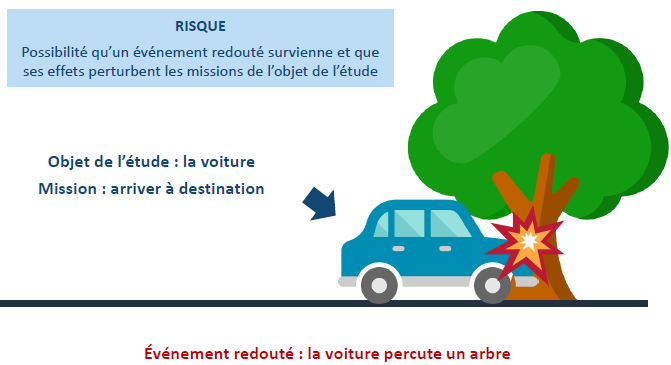
\includegraphics[scale=0.7]{./ressource/voiture1}
\end{center}

\begin{center}
 \rule{1.0\linewidth}{1pt}
 \end{center}

\begin{center}
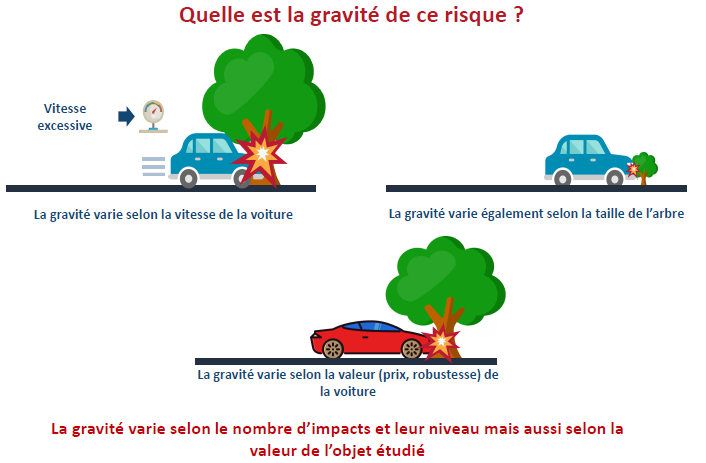
\includegraphics[scale=0.7]{./ressource/voiture2}
\end{center}
\begin{center}
 \rule{1.0\linewidth}{1pt}
 \end{center}
\begin{center}
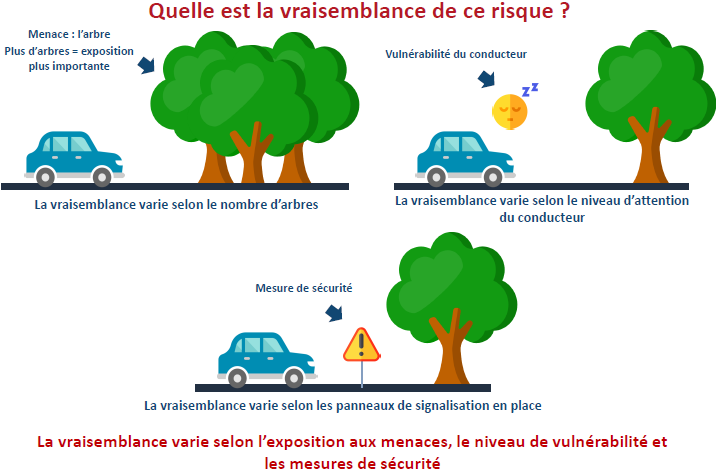
\includegraphics[scale=0.7]{./ressource/voiture3}
\end{center}
\begin{center}
 \rule{1.0\linewidth}{1pt}
 \end{center}
\begin{center}
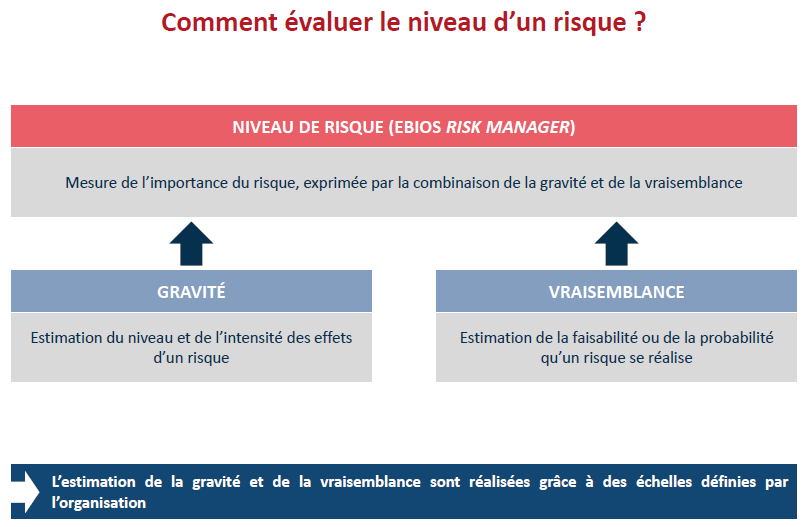
\includegraphics[scale=0.7]{./ressource/presentationRisqueManager}
\end{center}


\section{Méthode EBIOS Risk Manager}

La méthode \textbf{EBIOS Risk Manager} (Expression des Besoins et Identification des Objectifs de Sécurité) est développée par l'ANSSI. Elle vise à évaluer et traiter les risques de cybersécurité dans une organisation en alignant les enjeux métiers et les objectifs de sécurité.

Elle permet de 
\begin{enumerate}
    \itemE Permettre aux organisations de gérer efficacement leurs risques cyber.
    \itemE Favoriser un dialogue entre métiers et experts en sécurité.
    \itemE S'adapter à des contextes variés : réglementaire, technique ou organisationnel.
\end{enumerate}

\vspace{0.5cm}
La méthode EBIOS Risk Manager est une approche pour gérer les risques numériques. Elle combine deux approches complémentaires :
\begin{itemize}
\itemE \textbf{Conformité} : Mettre en place un socle de sécurité basé sur des normes ou standards pour gérer les risques "classiques" (accidentels ou environnementaux).
\itemE \textbf{Scénarios} : Étudier des scénarios spécifiques pour évaluer les risques liés à des menaces intentionnelles, comme les cyberattaques.
\end{itemize}

Ces deux approches travaillent ensemble, la conformité posant les bases nécessaires, et les scénarios ciblant les risques les plus sophistiqués. La démarche est représentée par une pyramide symbolisant cette progression et cette complémentarité.

\begin{center}
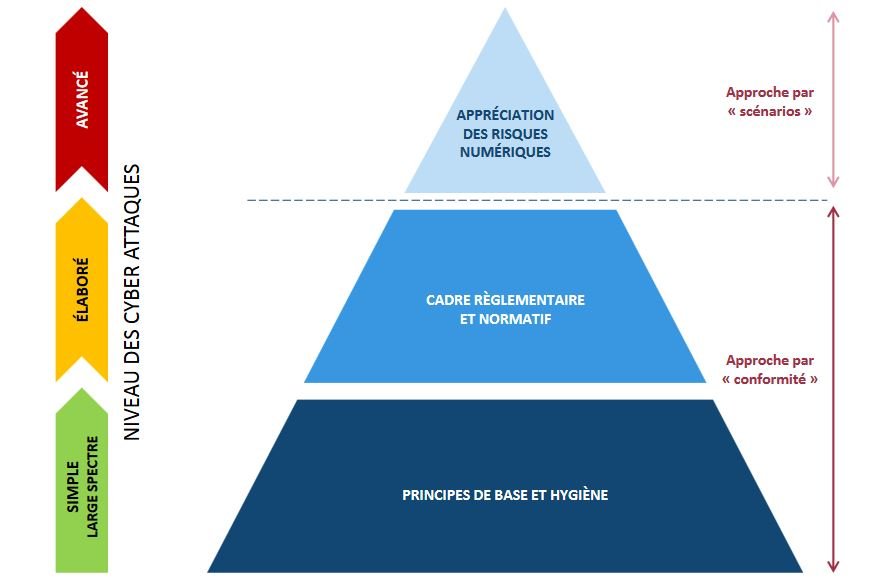
\includegraphics[scale=0.4]{./ressource/la pyramide.JPG}
\end{center}



\subsection*{Les cinq ateliers de la méthode}

La méthode est structurée autour de cinq ateliers collaboratifs :


\begin{center}
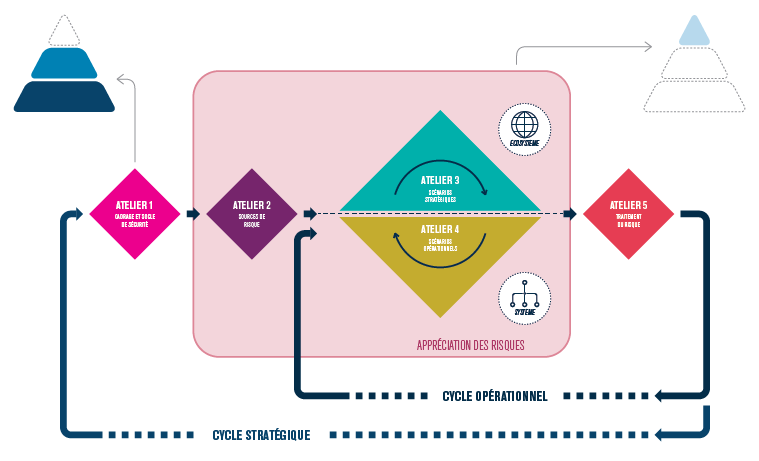
\includegraphics[scale=0.7]{./ressource/atelierIterative.png}
\end{center}

\begin{enumerate}[label=\textbf{Atelier \arabic* :}, leftmargin=1.5cm]
    \item \textbf{Cadrage et contexte - Qu’est ce qui doit être protégé, et pourquoi ?} définir les périmètres d'analyse, les enjeux métiers et les besoins en sécurité.
    \item \textbf{Sources de risques - Qui est l’agresseur et pourquoi passe-t-il à l’acte ?} identifier les menaces principales, les parties prenantes et les scénarios d'attaque.
    \item \textbf{Scénarios de risques - Par où l’attaquant va-t-il agir ?} construire des scénarios plausibles en liant menaces, vulnérabilités et impacts.
    \item \textbf{Stratégie de traitement - Comment l’attaquant va-t-il agir ?} prioriser les risques et définir les mesures de sécurité adaptées.
    \item \textbf{Communication et validation - Quelle stratégie de sécurité au regard des risques identifiés ?} restituer les résultats aux parties prenantes pour décision.
\end{enumerate}



\section{Détails des ateliers}

\textbf{Pour les détails des différents ateliers, nous allons réaliser une analyse de risque sur une salle de concert. ATTENTION, la démarche sera présentée, mais l'analyse ne sera ni exhaustive ni complète. }

\subsection{Atelier 1 : Cadrage et contexte}
\begin{encadre}{Objectif}
Définir le cadre de l’étude et du projet, son périmètre métier et technique
\end{encadre}

\begin{center}
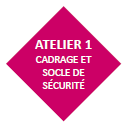
\includegraphics[scale=0.8]{./ressource/logoA1.png}
\end{center}


\paragraph{Eléments de sortie} - Répertoire : \href{run:./ressource_eleve/Atelier1/}{\verb?Atelier1?}
\begin{itemize}
    \itemE Éléments de cadrage de l’étude : participants, planning…
	\itemE Périmètre métier et technique : missions, valeurs métier, biens supports
		\begin{itemize}
		\item[+] \href{run:./ressource_eleve/Atelier1/A1_documents.ods}{Document A1\_documents.ods - A1\_01-perimetreMetier.ods}	
		\end{itemize}
	\itemE Événements redoutés et leur niveau de gravité 
		\begin{itemize}
		\item[+] \href{run:./ressource_eleve/Atelier1/A1_documents.ods}{Document A1\_documents.ods - A1\_02-evenementRedoute}	
		\end{itemize}
	\itemE Socle de sécurité : liste des référentiels applicables, état d’application, identification des écarts
		\begin{itemize}
		\item[+] \href{run:./ressource_eleve/Atelier1/A1_documents.ods}{Document A1\_documents.ods - A1\_03-regeleHygieneSecurite}	
		\end{itemize}
\end{itemize}
%%%%%%%%%%%%%%%%%%%%%
\vspace{0.5cm}
\begin{center}
 \rule{0.75\linewidth}{1pt}
\end{center}
\begin{minipage}[c]{0.59\linewidth}

\textbf{Tous les documents sont complétés $\Rightarrow$ Fin de l'atelier 1}
\end{minipage}
\begin{minipage}[c]{0.4\linewidth}
\begin{center}

\includegraphics[scale=0.1]{./ressource/OKLogo}
\end{center}
\end{minipage}
\begin{center}
 \rule{0.75\linewidth}{1pt}
\end{center}
%%%%%%%%%%%%%%%%%%%%%

\subsection{Atelier 2 : Sources de risques}
\begin{encadre}{Objectif}
Identifier les \textbf{Sources de Risque} (SR) et leurs \textbf{Objectifs Visés} (OV) en lien avec l’objet de l’étude
\end{encadre}

\begin{minipage}[c]{0.6\linewidth}
\paragraph{Eléments d'entrée}
\begin{itemize}
\itemE \href{run:./ressource_eleve/Atelier1/A1_documents.ods}{Valeurs métier (atelier 1) (Ex : gestion clients)}
\itemE \href{run:./ressource_eleve/Atelier1/A1_documents.ods}{Événements redoutés (atelier 1) (Ex : Falsification des indicateurs de la qualité de l'air)}
\end{itemize}
\end{minipage}
\begin{minipage}[c]{0.4\linewidth}
\begin{center}
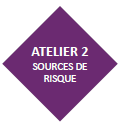
\includegraphics[scale=0.8]{./ressource/logoA2.png}
\end{center}
\end{minipage}



\paragraph{Eléments de sortie} - Répertoire : \href{run:./ressource_eleve/Atelier2/}{\verb?Atelier2?}
\begin{itemize}
	\itemE  Liste des couples SR/OV retenus pour la suite de l’étude
		\begin{itemize}
		\item[+] \href{run:./ressource_eleve/Atelier2/A2_documents.ods}{Document A2\_documents.ods - Feuille A2\_00-Identifier\_SR\_OV}
		\end{itemize}
	\itemE  Liste des couples SR/OV secondaires, qui seront si possible mis sous surveillance
		\begin{itemize}
		\item[+] \href{run:./ressource_eleve/Atelier2/A2_documents.ods}{Document A2\_documents.ods - Feuille A2\_01-Selection\_couple\_SR\_OV}
		\end{itemize}
	\itemE  Représentation des SR/OV sous la forme d’une cartographie
		\begin{itemize}
		\item[+] \href{run:./ressource_eleve/Atelier2/A2_documents.ods}{Document A2\_documents.ods - Feuille A2\_01-Selection\_couple\_SR\_OV}
		\end{itemize}
\end{itemize}

%%%%%%%%%%%%%%%%%%%%%
\vspace{0.5cm}
\begin{center}
 \rule{0.75\linewidth}{1pt}
\end{center}
\begin{minipage}[c]{0.59\linewidth}

\textbf{Tous les documents sont complétés $\Rightarrow$ Fin de l'atelier 2}
\end{minipage}
\begin{minipage}[c]{0.4\linewidth}
\begin{center}

\includegraphics[scale=0.1]{./ressource/OKLogo}
\end{center}
\end{minipage}
\begin{center}
 \rule{0.75\linewidth}{1pt}
\end{center}
%%%%%%%%%%%%%%%%%%%%%

\subsection{Atelier 3 : Scénarios de risques}
\begin{encadre}{Objectif}
Identifier les parties prenantes critiques de l’écosystème et construire des scénarios de
risque de haut niveau (scénarios stratégiques)
\end{encadre}


\begin{minipage}[c]{0.6\linewidth}
\paragraph{Eléments d'entrée}
\begin{itemize}
\itemE \href{run:./ressource_eleve/Atelier1/A1_documents.ods}{Missions et valeurs métier (atelier 1)}
\itemE \href{run:./ressource_eleve/Atelier1/A1_documents.ods}{Événements redoutés et leur gravité (atelier 1)}
\itemE \href{run:./ressource_eleve/Atelier2/A2_documents.ods}{Sources de risque et objectifs visés retenus (atelier 2)}
\end{itemize}

\end{minipage}
\begin{minipage}[c]{0.4\linewidth}
\begin{center}
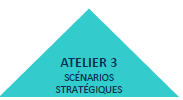
\includegraphics[scale=0.8]{./ressource/logoA3.png}
\end{center}
\end{minipage}



\paragraph{Élément de sortie} - Répertoire : \href{run:./ressource_eleve/Atelier3/}{\verb?Atelier3?}
\begin{itemize}
    \itemE Cartographie de menace de l’écosystème
    	\begin{itemize}
		\item[+] \href{run:./ressource_eleve/Atelier3/A3_documents.ods}{Document A3\_documents.ods - Feuille A3\_00-Cartographie}	
		\end{itemize}
	\itemE Scénarios stratégiques
		\begin{itemize}
		\item[+] \href{run:./ressource_eleve/Atelier3/A3_documents.ods}{Document A3\_documents.ods - Feuille A3\_01-Synthese}
		\end{itemize}
 	\itemE Mesures de sécurité retenues pour l’écosystème
 		\begin{itemize}
		\item[+] \href{run:./ressource_eleve/Atelier3/A3_documents.ods}{Document A3\_documents.ods - Feuille A3\_02-mesureSecurite}
		\end{itemize}
\end{itemize}

%%%%%%%%%%%%%%%%%%%%%
\vspace{0.5cm}
\begin{center}
 \rule{0.75\linewidth}{1pt}
\end{center}
\begin{minipage}[c]{0.59\linewidth}

\textbf{Tous les documents sont complétés $\Rightarrow$ Fin de l'atelier 3}
\end{minipage}
\begin{minipage}[c]{0.4\linewidth}
\begin{center}

\includegraphics[scale=0.1]{./ressource/OKLogo}
\end{center}
\end{minipage}
\begin{center}
 \rule{0.75\linewidth}{1pt}
\end{center}
%%%%%%%%%%%%%%%%%%%%%









\subsection{Atelier 4 : scénarios opérationnels}
\begin{encadre}{Objectif}
Construire les scénarios opérationnels schématisant les modes opératoires techniques qui  seront mis en oeuvre par les sources de risque
\end{encadre}

\begin{minipage}[c]{0.6\linewidth}
\paragraph{Eléments d'entrée}
\begin{itemize}
\itemE \href{run:./ressource_eleve/Atelier1/A1_documents.ods}{Missions, valeurs métier et biens supports (atelier 1)}
\itemE \href{run:./ressource_eleve/Atelier1/A1_documents.ods}{Socle de sécurité (atelier 1) }
\itemE \href{run:./ressource_eleve/Atelier2/A3_documents.ods}{Sources de risque et objectifs visés retenus (atelier 2)}
\itemE \href{run:./ressource_eleve/Atelier3/A3_documents.ods}{Scénarios stratégiques retenus (atelier 3)}
\end{itemize}

\end{minipage}
\begin{minipage}[c]{0.4\linewidth}
\begin{center}
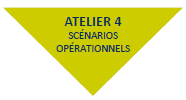
\includegraphics[scale=0.8]{./ressource/logoA4.png}
\end{center}
\end{minipage}





\paragraph{Élément de sortie} - Répertoire : \href{run:./ressource_eleve/Atelier4/}{\verb?Atelier4?}
\begin{itemize}
    \itemE Scénarios opérationnels
    	\begin{itemize}
		\item[+] \href{run:./ressource_eleve/Atelier4/A4_documents.ods}{Document A4\_documents.ods - Feuille A4\_00-scenario}
		\end{itemize}
	\itemE Évaluation des scénarios opérationnels en termes de vraisemblance
\end{itemize}

%%%%%%%%%%%%%%%%%%%%%
\vspace{0.5cm}
\begin{center}
 \rule{0.75\linewidth}{1pt}
\end{center}
\begin{minipage}[c]{0.59\linewidth}

\textbf{Tous les documents sont complétés $\Rightarrow$ Fin de l'atelier 4}
\end{minipage}
\begin{minipage}[c]{0.4\linewidth}
\begin{center}

\includegraphics[scale=0.1]{./ressource/OKLogo}
\end{center}
\end{minipage}
\begin{center}
 \rule{0.75\linewidth}{1pt}
\end{center}
%%%%%%%%%%%%%%%%%%%%%









\subsection{Atelier 5 : traitement du risque}
\begin{encadre}{Objectif}
Définir une stratégie de traitement du risque et identifier les risques résiduels
\end{encadre}


\begin{minipage}[c]{0.6\linewidth}
\paragraph{Eléments d'entrée}
\begin{itemize}
%\href{run:./ressource_eleve/AtelierX/AX_documents.ods'}{AX\_documents.ods}
    \itemE \href{run:./ressource_eleve/Atelier1/AX_documents.ods}{Socle de sécurité (atelier 1)}
    \itemE \href{run:./ressource_eleve/Atelier3/A3_documents.ods}{Mesures de sécurité portant sur l’écosystème (atelier 3)}
    \itemE \href{run:./ressource_eleve/Atelier3/A3_documents.ods}{Scénarios stratégiques (atelier 3)}
	\itemE \href{run:./ressource_eleve/Atelier4/A4_documents.ods}{Scénarios opérationnels (atelier 4)}
\end{itemize}

\end{minipage}
\begin{minipage}[c]{0.4\linewidth}
\begin{center}
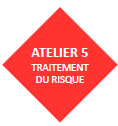
\includegraphics[scale=0.8]{./ressource/logoA5.png}
\end{center}
\end{minipage}


\paragraph{Élément de sortie} - Répertoire : \href{run:./ressource_eleve/Atelier5/}{\verb?Atelier5?}
\begin{itemize}
    \itemE Scénarios opérationnels
    	\begin{itemize}
		\item[+] \href{run:./ressource_eleve/Atelier5/A5_documents.ods'}{Document A5\_documents.ods - Feuille A5\_00-scenario}		
		\end{itemize}
	\itemE Plan d’amélioration continue de la sécurité (PACS) 
		\begin{itemize}
		\item[+]  \href{run:./ressource_eleve/Atelier5/A5_documents.ods}{Document A5\_documents.ods - Feuille A5\_01-PlanAmeliorationContinueSecu(PACS)}
		\end{itemize}
	\itemE Synthèse des risques résiduels
		\begin{itemize}
		\item[+] \href{run:./ressource_eleve/Atelier5/A5_documents.ods}{Document A5\_documents.ods - Feuille A5\_02-RisquesResiduels}		
		\end{itemize}
	\itemE Cadre du suivi des risques
		\begin{itemize}
		\item[+]Non réalisé pour cet exercice
		\end{itemize}
	
\end{itemize}






\section{Conclusion}

La méthode EBIOS Risk Manager est un outil puissant pour maîtriser les risques cyber tout en intégrant les objectifs stratégiques de l'organisation. En appliquant rigoureusement ses principes, une organisation peut anticiper les menaces, protéger ses actifs critiques et renforcer sa résilience.

\paragraph{Avantages :}
\begin{itemize}
    \itemE Approche collaborative, favorisant l'engagement des parties prenantes.
    \itemE Alignement entre stratégie métier et sécurité.
    \itemE Adaptabilité à différents contextes.
\end{itemize}

\paragraph{Limites :}
\begin{itemize}
    \itemE Nécessite une animation experte pour les ateliers.
    \itemE Demande un investissement initial important en temps et en ressources.
\end{itemize}


\paragraph{Ressources complémentaires :}
\begin{itemize}
    \itemE \href{https://www.ssi.gouv.fr}{Site officiel de l'ANSSI}
    \itemE \href{https://www.ssi.gouv.fr/guide-ebios-risk-manager/}{Documentation complète EBIOS Risk Manager}
\end{itemize}


\end{document}
